\documentclass[pdf]{beamer}
%\mode<presentation>{}

\usepackage{amssymb,amsmath,amsthm,enumerate}
\usepackage[utf8]{inputenc}
\usepackage{array}
\usepackage[parfill]{parskip}
\usepackage{graphicx}
\usepackage{caption}
\captionsetup[figure]{labelformat=empty}
\usepackage{subcaption}
\usepackage{bm}
\usepackage{amsfonts,amscd}
%\usepackage{gensymb}
\usepackage[]{units}
\usepackage{listings}
\usepackage{multicol}
\usepackage{tcolorbox}
\usepackage{physics}
\usepackage{multimedia} % movies!
\usepackage[export]{adjustbox} % crop graphics

\usepackage{pgfpages}
\usepackage{ifthen} % package required
\usepackage[subpreambles=true]{standalone}
\usepackage{appendixnumberbeamer}
\usepackage{rotating}

\setbeameroption{show notes on second screen}

%new commands
\newcommand{\der}[2]{\frac{d#1}{d#2}}
\newcommand{\nder}[3]{\frac{d^#1 #2}{d #3 ^ #1}}
\newcommand{\pder}[2]{\frac{\partial #1}{\partial #2}}
\newcommand{\npder}[3]{\frac{\partial ^#1 #2}{\partial #3^#1}}
\newcommand{\sentencelist}{def}
\newcommand{\overbar}[1]{\mkern 1.5mu\overline{\mkern-1.5mu#1\mkern-1.5mu}\mkern 1.5mu}
\newcommand{\lined}{\overbar}
\newcommand{\perm}[2]{{}^{#1}\!P_{#2}}
\newcommand{\comb}[2]{{}^{#1}C_{#2}}
\newcommand{\intall}{\int_{-\infty}^{\infty}}
\newcommand{\Var}[1]{\text{Var}\left(#1\right)}
\newcommand{\E}[1]{\text{E}\left(#1\right)}
\newcommand{\define}{\equiv}
\newcommand{\diff}[1]{\mathrm{d}#1}
\newcommand{\empy}[1]{{\color{darkorange}\emph{#1}}}
\newcommand{\empr}[1]{{\color{cardinalred}\emph{#1}}}


\theoremstyle{remark}
\newtheorem*{remark}{Remark}
\theoremstyle{definition}

\newcommand{\examplebox}[2]{
\begin{tcolorbox}[colframe=darkcardinal,colback=boxgray,title=#1]
#2
\end{tcolorbox}}

\newcommand{\eld}[1]{\frac{d}{dt}(\frac{\partial L}{\partial \dot #1}) - \frac{\partial L}{\partial #1}=0}
\newcommand{\euler}[1]{\frac{\partial L}{\partial #1}-\frac{d}{dt}(\frac{\partial L}{\partial \dot #1})}
\newcommand{\eulerg}[1]{\frac{\partial g}{\partial #1}-\frac{d}{dt}(\frac{\partial g}{\partial \dot #1})}
\newcommand{\divg}[1]{\nabla\cdot #1}
\newcommand{\prob}[1]{P(#1\vert I)}
\DeclareMathOperator*{\argmax}{argmax}

\beamertemplatenavigationsymbolsempty

\addtobeamertemplate{footnote}{\hskip -1.8em}{}

% ================================ %
%      Section dividers            %
\newboolean{sectiontoc}
\setboolean{sectiontoc}{true} % default to true
\AtBeginSection[]
{
  \ifthenelse{\boolean{sectiontoc}}{
    \begin{frame}<beamer>{Gliederung}
      \tableofcontents[currentsection]
    \end{frame}
  }
}

\newcommand{\sectionNoDivider}[1]{
  \setboolean{sectiontoc}{false}
  \section{#1}
  \setboolean{sectiontoc}{true}
}

% \newcommand<>{\makered}[1]{{\color#2{red}#1}}
% \renewcommand<>{\hyperlink}[2]{\only#3{\beameroriginal{\hyperlink}{#1}{#2}}}
\newcommand<>{\nakedfootnote}[1]{%
  \begingroup
  \renewcommand<>\thefootnote{}\footnote#2{#1}%
  \addtocounter{footnote}{-1}%
  \endgroup
}

\AtBeginSection[]
{
	\ifthenelse{\boolean{sectiontoc}}{
	  \begin{frame}<beamer>
	    \frametitle{\insertsectionhead}
	    \tableofcontents[currentsection,hideallsubsections]
	  \end{frame}
	}
}

\AtBeginSubsection[]
{
  \begin{frame}<beamer>
    \frametitle{Outline for \insertsectionhead}
    \tableofcontents[
        currentsection,
        currentsubsection,
        subsectionstyle=show/shaded/hide
    ]
  \end{frame}
}

\usetheme{Stanford}
\def \i  {\item}
\def \ai {\item[] \quad \arrowbullet}
\newcommand \si[1]{\item[] \quad \bulletcolor{#1}}
\def \wi {\item[] \quad $\ \phantom{\Rightarrow}\ $}
\def \bi {\begin{itemize}\item}
\def \ei {\end{itemize}}
\def \be {\begin{equation*}}
\def \ee {\end{equation*}}
\def \bie {$\displaystyle{}
\def \eie {{\ }$}}
\def \bsie {\small$\displaystyle{}
\def \esie {{\ }$}\normalsize\selectfont}
\def \bse {\small\begin{equation*}}
\def \ese {\end{equation*}\normalsize}
\def \bfe {\footnotesize\begin{equation*}}
\def \efe {\end{equation*}\normalsize}
\renewcommand \le[1] {\\ \medskip \lefteqn{\hspace{1cm}#1} \medskip}
\def \bex {\begin{example}}
\def \eex {\end{example}}
\def \bfig {\begin{figure}}
\def \efig {\end{figure}}
\def \btheo {\begin{theorem}}
\def \etheo {\end{theorem}}
\def \bc {\begin{columns}}
\def \ec {\end{columns}}
\def \btab {\begin{tabbing}}
\def \etab {\end{tabbing}\svneg\svneg}
\newcommand \col[1]{\column{#1\linewidth}}
\def\vneg  {\vspace{-5mm}}
\def\lvneg {\vspace{-10mm}}
\def\svneg {\vspace{-2mm}}
\def\tvneg {\vspace{-1mm}}
\def\vpos  {\vspace{5mm}}
\def\lvpos {\vspace{10mm}}
\def\svpos {\vspace{2mm}}
\def\tvpos {\vspace{1mm}}
\def\hneg  {\hspace{-5mm}}
\def\lhneg {\hspace{-10mm}}
\def\shneg {\hspace{-2mm}}
\def\thneg {\hspace{-1mm}}
\def\hpos  {\hspace{5mm}}
\def\lhpos {\hspace{10mm}}
\def\shpos {\hspace{2mm}}

\logo{
\includegraphics[height=0.5in]{./style_files_stanford/SU_New_BlockStree_2color.png}}



\title[\insertsectionhead]{data.0}
% \title[PhD Qualifying Exam]{Causal models of brain dynamics}
% \subtitle{Unsupervised learning of optogenetic experiments via deep generative models}



\begin{document}



\author[Tyler Benster, Qualifying Exam]{
	\begin{tabular}{c}
	\Large
	Tyler Benster\\
    \footnotesize
    Deisseroth and Druckmann Labs
\end{tabular}
\vspace{-2ex}
}

\institute{
	\vspace{2ex}
	
\includegraphics[height=0.4in]{./style_files_stanford/SU_New_BlockStree_2color.png}\\
	d-lab meeting\\
	}

\date{Sept 24, 2019}

\begin{noheadline}
\begin{frame}\maketitle\end{frame}
\end{noheadline}

%%%%%%%%%%%%%%%%%%%% Actual start %%%%%%%%%%%%%%%%%%%%%%%%%%%%%

\begin{frame}<beamer>
    \frametitle{Roadmap}
    \tableofcontents[subsectionstyle=hide]\
		\note[item]{I will first talk about why my overall goal is predicting neural activity, and discuss the importance of causal models as opposed to merely descriptive ones. I will further motivate this modeling goal by describing applications that are enabled by this approach.}
		\note[item]{In my first aim, I propose that a reasonable direction is to eschew biological plausibility and leverage state-of-art deep learning networks for predicting neural activity, and show that this approach outperforms current brain-wide modeling.}
		\note[item]{For my second aim, I propose a model-based approach to choosing optogenetic stimulation patterns such that we efficiently learn the best model parameters.}
		\note[item]{Finally, in my third aim, I suggest methods to incorporate biological priors as well as explicitly extract biological hypotheses.}
\end{frame}

\newcommand{\aimOne}{Aim 1: Spatial modeling with deep generative models}
\newcommand{\aimTwo}{Aim 2: Optogenetic active learning}
\newcommand{\aimThree}{Aim 3: Contribution of cell-types and circuit motifs}
\newcommand{\qOne}{What is the most effective approach to predict whole-brain observations?}
\newcommand{\qTwo}{How do we resolve model underdetermination?}
\newcommand{\qThree}{Do model substructures map to underlying biology?}

\begin{frame}{Whole-brain prediction facilitates construction of causal models}
  \begin{columns}[t]
    \column{0.31\textwidth}
    \uncover<1->{
      \resizebox{\textwidth}{!}{% \documentclass[tikz,crop]{standalone}
\documentclass[border=15pt, multi, tikz, ifthen, xcolor]{standalone}
\usepackage{tikz, xcolor, ifthen}
\usetikzlibrary{shapes,arrows}
\usetikzlibrary{positioning}

\begin{document}

\begin{tikzpicture}[node distance = 2cm, auto]
    \node [] (o1) {observations};
    \node [above=5mm of o1] (m1) {model};
    \node [above=5mm of m1] (b1) {biology};
    \path [line] (b1) -- (m1);
    \path [line] (m1) -- (o1);
\end{tikzpicture}
\end{document}
}
    }
    \column{0.65\textwidth}
    \only<2>{
      \resizebox{\textwidth}{!}{% \documentclass[tikz,crop]{standalone}
\documentclass[border=15pt, multi, tikz, ifthen, xcolor]{standalone}
\usepackage{tikz, xcolor, ifthen}
\usetikzlibrary{shapes,arrows}
\usetikzlibrary{positioning}

\begin{document}

\begin{tikzpicture}[node distance = 2cm, auto]
    \node [] (o1) {observations};
    \node [right=2mm of o1] (b1) {biology prior};
    \node [below right=5mm and -3mm of o1] (m1) {model};
    \node [below=5mm of m1] (b2) {biology posterior};
    \path [line] (o1) -- (m1);
    \path [line,dashed] (b1) -- (m1);
    \path [line,dashed] (m1) -- (b2);
\end{tikzpicture}
\end{document}
}
    }
    \only<3->{
      \resizebox{\textwidth}{!}{% \documentclass[tikz,crop]{standalone}
\documentclass[border=15pt, multi, tikz, ifthen, xcolor]{standalone}
\usepackage{tikz, xcolor, ifthen}
\usetikzlibrary{shapes,arrows}
\usetikzlibrary{positioning}

\begin{document}

\begin{tikzpicture}[node distance = 2cm, auto]
    \node [] (o1) {\emph{do}(observations)};
    \node [right=2mm of o1] (b1) {biology prior};
    \node [below right=5mm and -3mm of o1] (m1) {model};
    \node [below=5mm of m1] (b2) {biology posterior};
    \path [line] (o1) -- (m1);
    \path [line,dashed] (b1) -- (m1);
    \path [line,dashed] (m1) -- (b2);
\end{tikzpicture}
\end{document}
}
    }
  \end{columns}
  \uncover<4->{
    \begin{itemize}
      \item Observing whole-brain $\rightarrow$ fewer latent variables
      \item Interventions enable building causal model
      \item Causal models aid applications and interpretations
    \end{itemize}
  }
  \note[item]{Data-driven approach may result in empirically more accurate model.}
    \note<4->[item]{Behavior is encoded by populations of neurons distributed across whole-brain.}
\end{frame}

\begin{frame}{\aimOne}
  \textbf{\qOne}
  \begin{itemize}
    \item State-of-art performance in video prediction is achieved by deep generative models
    \item Collected preliminary brain-wide calcium data during an optomotor behavior
    \item Initial modeling results suggest that spatial modeling out-performs traditional point process models of neurons
  \end{itemize}
\end{frame}

\begin{frame}{\aimTwo}
  \textbf{\qTwo}
  \begin{itemize}
    \item For complex models fit to finite observations, multiple choices of parameters may perform equally well
    \item We can resolve this by testing if model substructures are causal with optogenetics
    \item First experiment failed due to poor optogenetic activation, but a new more-sensitive opsin will make the experiment easier
  \end{itemize}
\end{frame}

\begin{frame}{\aimThree}
  \textbf{\qThree}
  \begin{itemize}
    \item \emph{in situ} hybridization (ISH) and connectome data contribute to understanding of colored graphs that underlie functional observations
    \item First attempt to add excitatory and inhibitory staining as an additional model input modestly hurt performance
    \item Training model to predict ISH data will force model to maintain representation of cell type
    \item Known circuit motifs can be used as a prior, or we can try to discover structure using structure active learning
  \end{itemize}
\end{frame}

\section{Motivation \& Background}


\begin{frame}[t]{The probability distribution revolution}
	\begin{multicols}{2}
		\begin{itemize}
			\item Karl Pearson (1857-1936) came with the idea that scientific measurements should be conceived as coming from probability distributions.
			\item Scientific measurements are just random reflections of the underlying truth that is the distribution.
			\item “A great book on the
history of statistics” $\rightarrow$ Aaron
			\item
		\end{itemize}

		\columnbreak

		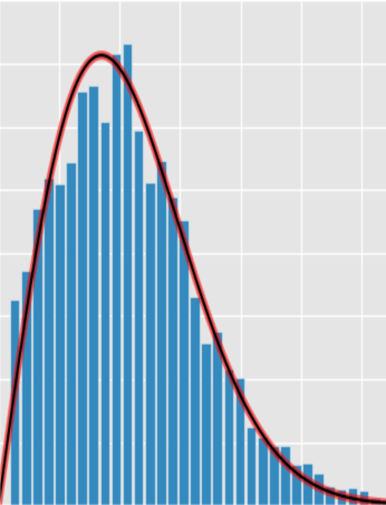
\includegraphics[width=0.25\textwidth]{media/distribution}
		\linebreak
		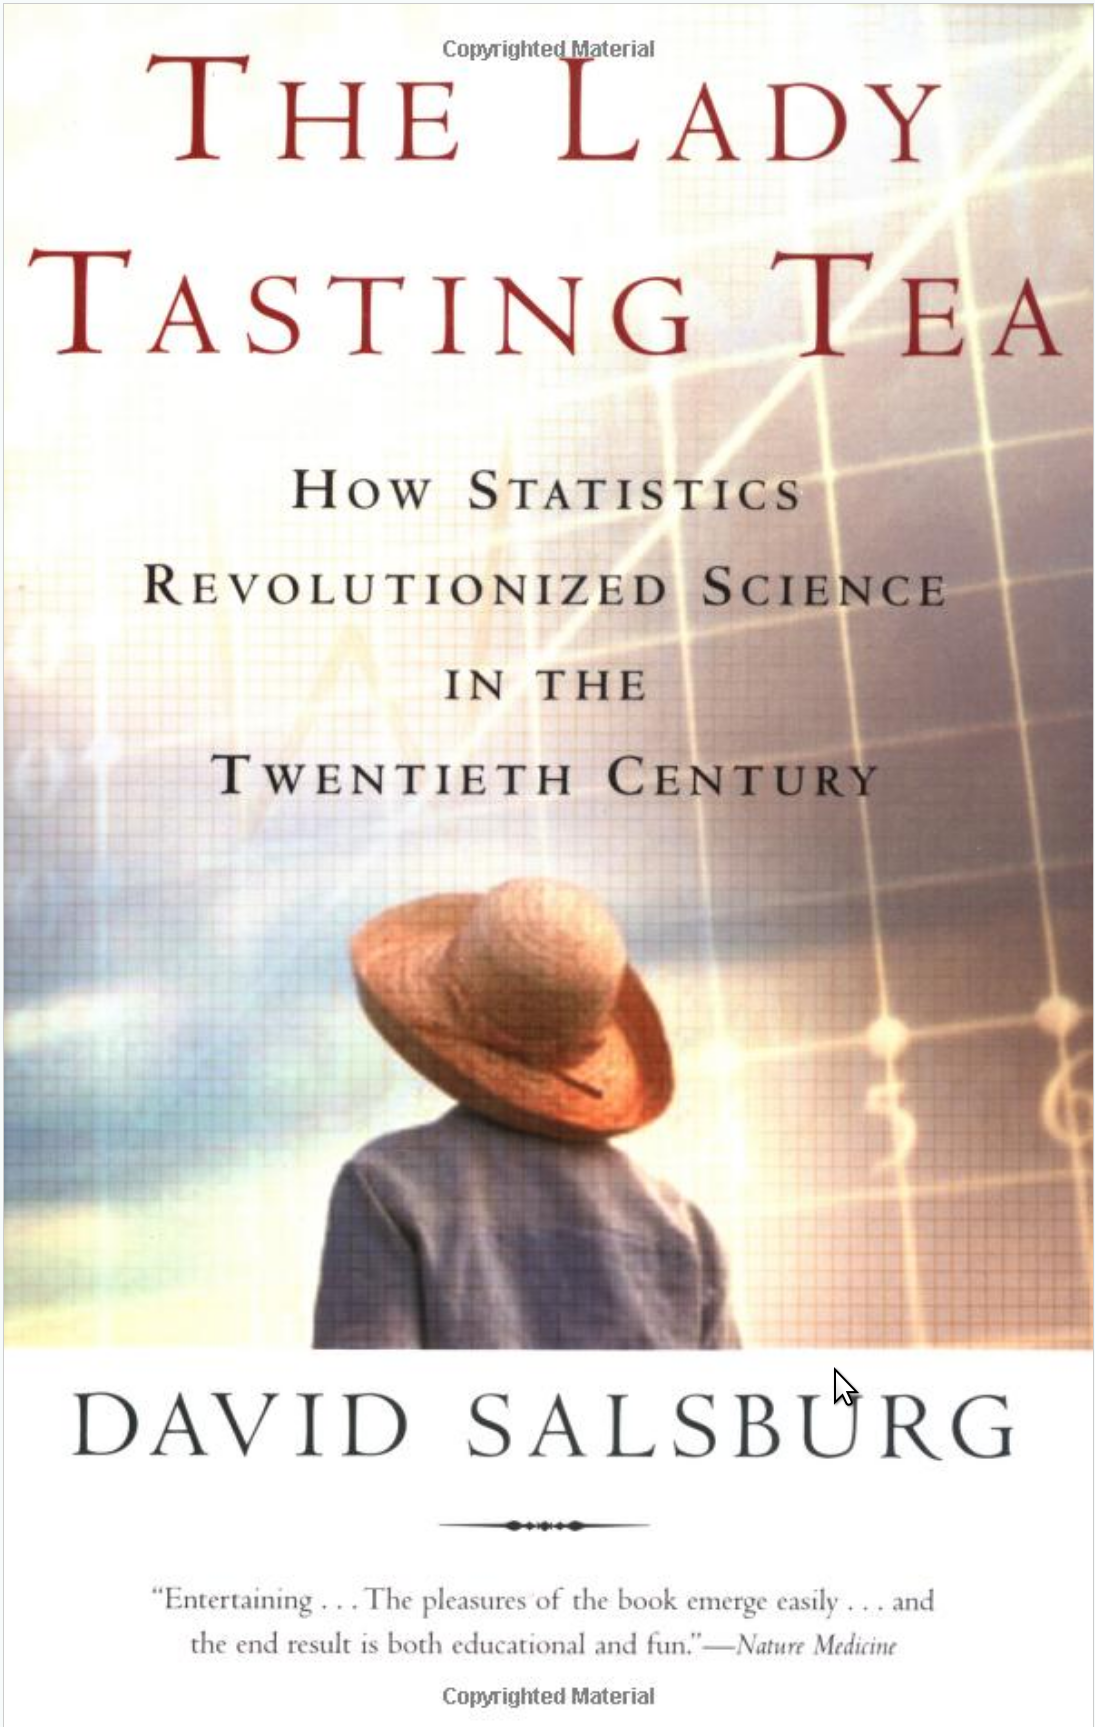
\includegraphics[width=0.25\textwidth]{media/book}
	\end{multicols}

	\note{Lets start with a bit of history. The idea that scientific measurements are best understood as reflecting underlying probabilities distributions is a relatively new idea.

It was a now famous thinker and scientist, Karl Pearson (of the Pearson correlation coefficient) who conceived the idea in late 18 hundreds.

He realized randomness was inherent part of nature and of scientific measure, and he formulated the idea that all measurments should be conceived of as coming from an underlying probability distributions.

In other words, the underlying truth is the distrubutions, and the measurements are just random reflections of this truth.  At the time, this was a revolutionary idea.}
\end{frame}

\begin{frame}[t]{The power of probability distributions}
	Distributions allow scientists to:
	\begin{itemize}
		\item Understand scientific measurement
		\item Predict the probability of specific data
		\item Test specific hypothesis (p-values)
		\item Produce generative models
		\item Better conceptual understanding data.
	\end{itemize}
	\note{And it was an idea that revolutized science.

	It allowed scientists to:
	\begin{itemize}
		\item Better understand their measurements.
		\item To make predictions about what data they should expect to observe.
		\item To test scientific hypotheses in a mathematically rigorous way.
		\item To build generative models of their data, and to test how well those models explain the observed measurments.
		\item And in general to have a better conceptual understanding of the data they generated.
	\end{itemize}
}
\end{frame}
%--- Next Frame ---%

\begin{frame}[t]{Estimating distributions from data}
	\begin{multicols}{2}
		Low-Dimensional:
		\begin{itemize}
			\item Great tools to fit and understand the underlying probability distribution of data.
		\end{itemize}
		\vfill\columnbreak
		High-Dimensional:
		\begin{itemize}
			\item In some cases, classical statistical tools are insufficient.
			\item Problematic for modern neuroscience: \begin{itemize}
				\item Thousands of electrodes.
				\item Millions of voxels.
			\end{itemize}
		\end{itemize}
	\end{multicols}
	\note{Since Pearson’s early work, scientists and statisticians have devised an enormous number of related tools.

For example they’ve defined many many distributions, and they’ve created tools for working with those distrubitons (calculating likelihoods and fitting them).

One class of tools aim to estimate the underlying distribution that generated an observed empirical measurment.

These tools are highly effective when data is low dimensional, but they are sometimes insufficient when data is high dimensional.}
\end{frame}
%--- Next Frame ---%

\begin{frame}[t]{How can we build statistical distributions for neuroscience datasets?}
	\movie[]{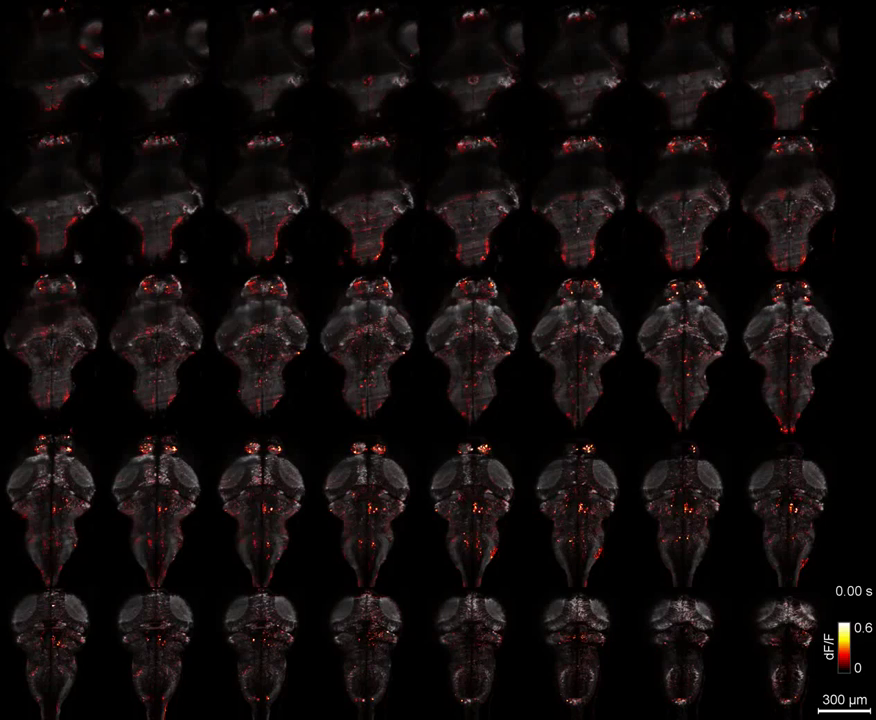
\includegraphics[width=0.7\textwidth,center]{media/zfish_first.png}}{media/zfish_imaging.mp4}
	\nakedfootnote{\url{https://www.youtube.com/watch?v=CXYp9xCUhe0}}
	\note{For example, consider whole brain imaging data from the zebrafish.  This data can have millions of dimensions, which makes estimating the understanding joint probability distribution difficult.  The number of possible states is enormous.  The voxels are not independent.  You can’t simply make a histogram or a heat-map.
			}
\end{frame}

\section{\aimOne}

\begin{frame}{\qOne}
	\textbf{Hypothesis:} deep learning spatial models will outperform point process models
	\begin{itemize}
		\item Extract neuron fluorescent traces $\rightarrow$ build RNN
		\item Raw fluorescent observations $\rightarrow$ convolutional deep learning model
		\item Compare prediction performance on withheld test data
	\end{itemize}
\end{frame}

\note{
	The main buy-in for this talk is that having an  accurate model of brain dynamics is useful. Most approaches today for brain-wide modeling use hand-crafted features in a  preprocessing pipeline that throws away spatial information. How much better can we do at predicting activity if we do not constrain our modeling by biological plausibility?
}

\begin{frame}{ 2P Experimental setup }
	\centering
	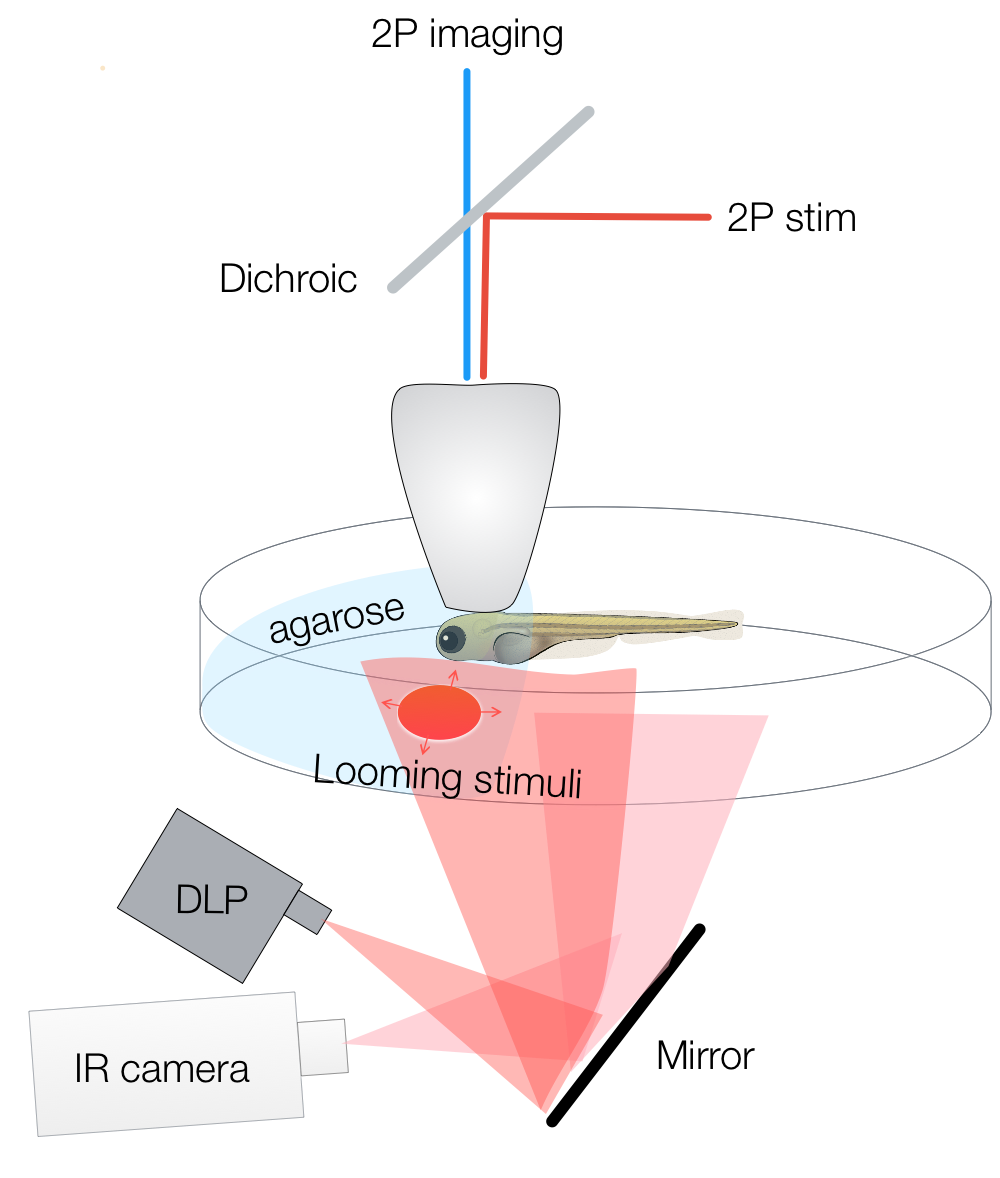
\includegraphics[height=\textheight]{media/experimental_setup.png}
\end{frame}{}

\begin{frame}{ Whole-brain 2P calcium imaging }{Z-projection of 19 planes, 4x real-time, 2Hz}
	% TODO make video shorter
	% center figure larger than textwidth
		\movie[]{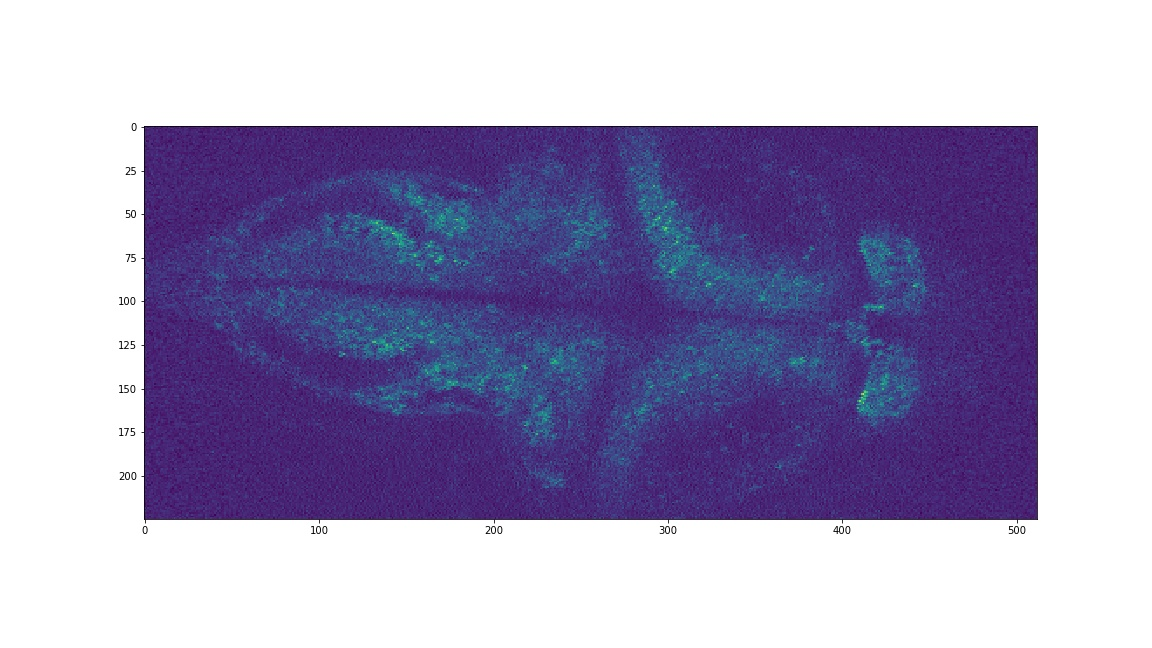
\includegraphics[width=0.6\textwidth,center]{media/20190429_f5e2.jpg}}{media/20190429_f5e2.mp4}
		\vspace{-20mm}
		\centering
		\begin{turn}{-90}
				\begin{minipage}{0.7\textheight}
					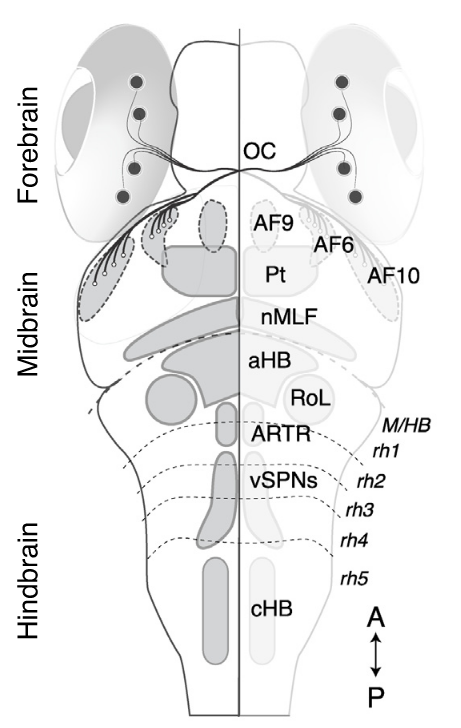
\includegraphics[height=0.5\textheight]{media/larval_atlas}
			 \end{minipage}
		 \end{turn}

	 % 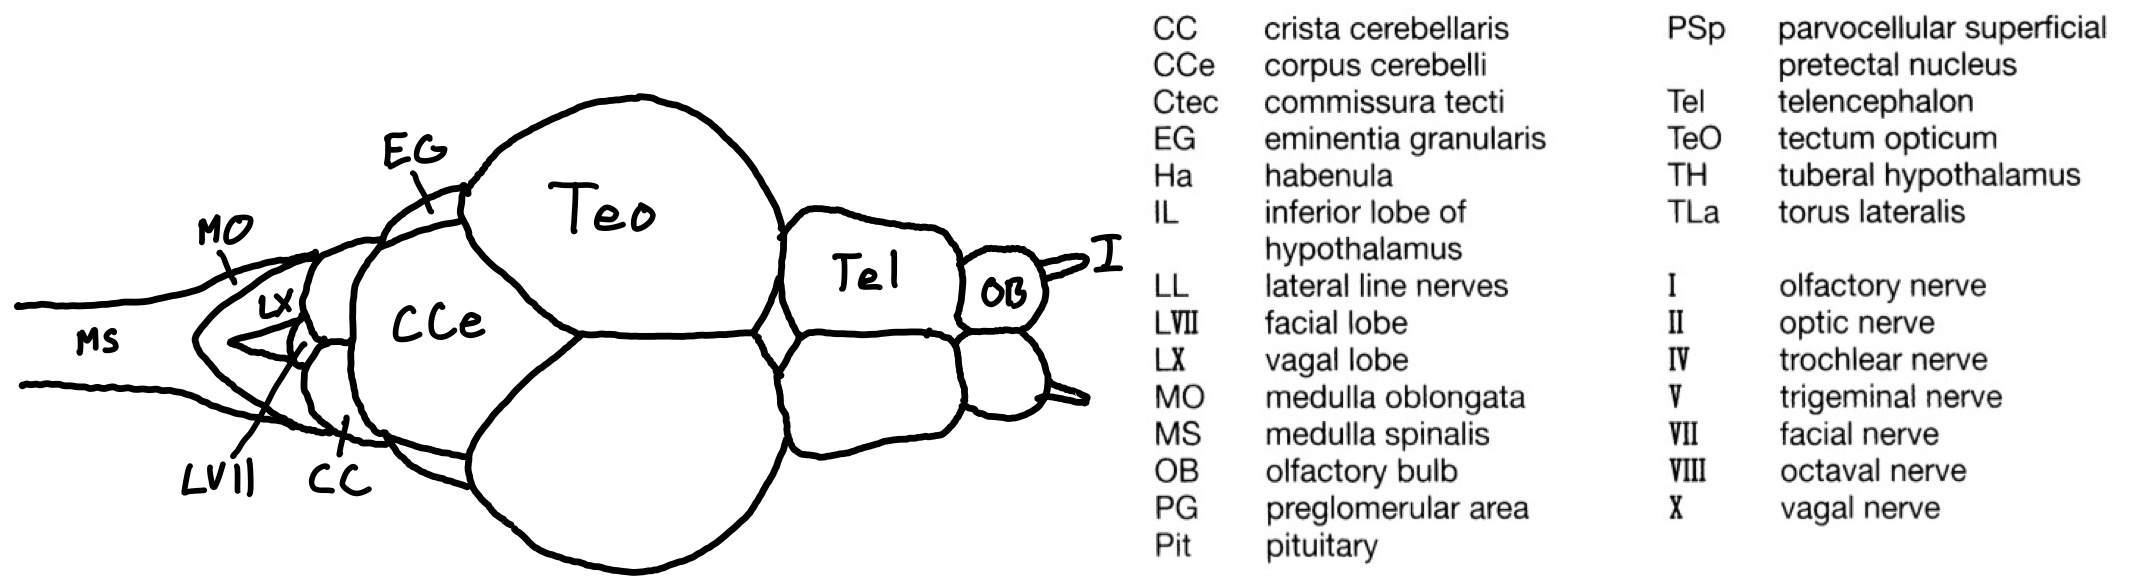
\includegraphics[height=0.5\textheight]{media/atlas}
	 \nakedfootnote{Naumann, Fitzgerald, et al. 2016}

	\note{need to change 2P offset for bidirectional imaging: ~2px jitter line-to-line}
	\note[item]{resting state video, no external stimuli}
	\note[item]{highlight brain deformation during tail movement}
	\note[item]{This is a video. About 2/3 way through, brain goes completely dark (!!), then whole brain lights up.}
\note[item]{Dorsal overview of zebrafish neuroanatomy. DSRGCs (black dots) project via the optic chiasm (OC) to ten contralateral retinal arborization fields(AFs). Pt,pretectum; nMLF, nucleus of the medial longitudinal fasciculus; aHB, anterior hindbrain; RoL, neurons in rhombomere 1; ARTR, anterior rhombencephalic turningregion; vSPNs, ventromedial spinal projection neurons; cHB, caudal hindbrain; M/HB, midbrain-hindbrain border; rh1–5, rhombomeres 1–5. A, anterior; P,posterior.}
\end{frame}


\begin{frame}{ Current approaches to brain-wide modeling }
	% \setcounter{footnote}{1}
	\begin{multicols}{2}
		\adjincludegraphics[width=0.6\textwidth,trim={0 {.42\height} 0 0},clip]{media/caiman.jpg}
		Extract neuron traces\nakedfootnote{Giovannucci et al. 2019.}
		\note<1>{In the early days of machine vision, researchers often used handcrafted feature extracters like edge detection to extract lower dimensional features that are then fed into a model. Today, neuroscience is similar: we motion correct a raw movie, identify independent spatial components, separate the sources, and attempt to whiten the signal based on assumptions of calcium indicator dynamics.}
		\vfill\null\columnbreak
		\uncover<2>{
			\adjincludegraphics[width=0.4\textwidth,trim={0 {.7\height} {.65\width} 0},clip]{media/kanaka.jpg}
			\,
			Add back spatial information
		}
	\end{multicols}
	% \begin{columns}[t]
	% 	\begin{column}{0.6\textwidth}
	% 		\adjincludegraphics[width=\textwidth,trim={0 {.42\height} 0 0},clip]{media/caiman.jpg}
	% 		Extract neuron traces\nakedfootnote{Giovannucci et al. 2019.}
	% 		\note<1>{In the early days of machine vision, researchers often used handcrafted feature extracters like edge detection to extract lower dimensional features that are then fed into a model. Today, neuroscience is similar: we motion correct a raw movie, identify independent spatial components, separate the sources, and attempt to whiten the signal based on assumptions of calcium indicator dynamics.}
	% 		% \vfill\null\columnbreak
	% 	\end{column}
	% 	\begin{column}{0.4\textwidth}
	% 		\uncover<2>{
	% 			\adjincludegraphics[width=\textwidth,trim={0 {.7\height} {.65\width} 0},clip]{media/kanaka.jpg}
	% 			\,
	% 			Add back spatial information
	% 		}
	% 	\end{column}
	% \end{columns}
	\note<2>{In general, modeling a recurrent neural network is intractable as the number of parameters grows quadradically with a number of neurons. Thus, brain-wide modeling usually involves a sparsity prior based on spatial location. In the neuroscience literature, it is not yet the norm to evaluate performance of modeling on held-out test data so we typically evaluate modeling based on how well it matches previous findings in the literature.}
	\nakedfootnote<2>{Andalman et al. 2019.}
\end{frame}{}

\begin{frame}{ Latent-space volume prediction  }{Stochastic embedding}
	% \adjincludegraphics[width=\textwidth,trim={0 {0.35\height} 0 0},clip]{media/my_architecture.png}
	\resizebox{\textwidth}{!}{% \documentclass[tikz,crop]{standalone}
\documentclass[border=15pt, multi, tikz, pgfmath, ifthen, xcolor]{standalone}
\usepackage{tikz, xcolor, pgfmath, ifthen}
\usetikzlibrary{shapes,arrows}
\usetikzlibrary{positioning}

\tikzstyle{decision} = [diamond, draw, text width=4.5em,
                        text badly centered, node distance=2cm,
                        inner sep=0pt]
\tikzstyle{block} = [rectangle, draw, text width=5em,
                     text centered, rounded corners,
                     minimum height=4em, node distance=3cm]
\tikzstyle{line} = [draw, -latex']
\tikzstyle{cloud} = [draw, ellipse, node distance=2.5cm, minimum height=2em]
\tikzstyle{blank} = [node distance=1cm]

\tikzstyle{square} = [regular polygon,regular polygon sides=4]

\tikzstyle{var} = [minimum size=2em]
\tikzstyle{random} = [circle, minimum width=10mm, draw, inner sep=0pt, font=\scriptsize]
\tikzstyle{rnn} = [square, minimum width=12mm, minimum height=2mm, draw, inner sep=0pt, font=\scriptsize]
\tikzstyle{encoder} = [trapezium, minimum width=10mm, minimum height=6mm, trapezium angle=60,
                        inner sep=0pt, draw, font=\scriptsize]

\begin{document}
\def\xtime{{"t-2","t-1","t","t+1","t+2","t+3"}}

% one day: draw stack https://tex.stackexchange.com/questions/171998/stack-figures-in-horizontal-plane-in-3d-rectangular-shape-without-loss-of-qualit
\begin{tikzpicture}[node distance = 2cm, auto]
    \foreach \t [count=\n,evaluate=\n as \mytime using ({\xtime[int(\n-1)]})] in {-2,-1,0} {
        % Place nodes
        \pgfmathsetmacro{\num}{int(\t-1)}
        \ifthenelse{\n=1}
            {\node [var] (x\t) {$x_{\mytime}$};}
            {\node [var, right=8mm of xh\num] (x\t) {$x_{\mytime}$};}
        \node [var, right=8mm of x\t] (xh\t) {$\hat{x}_{\mytime}$};

        \node [encoder, above=6mm of x\t] (e\t) {e};
        \node [encoder, above=6mm of xh\t] (d\t) {d};

        \node [random, above right=6mm and 1.5mm of e\t] (z\t) {$z_{\mytime}$};
        \node [rnn, above=6mm of z\t] (r\t) {RNN};
        \node [var, above=6mm of r\t] (c\t) {$c_{\mytime}$};

        % Draw edges
        \path [line] (x\t) -- (e\t);
        \path [line] (e\t) -- (z\t);
        \path [line] (z\t) -- (r\t);
        \path [line] (r\t) -- (c\t);
        \path [line] (z\t) -- (d\t);
        \path [line] (d\t) -- (xh\t);
        \ifthenelse{\n=1}
            {}
            {\path [line] (r\num) -- (r\t);}
    }

    \foreach \t [count=\n,evaluate=\n as \mytime using ({\xtime[int(\n+2)]})] in {1,2,3} {
        % Place nodes
        \pgfmathsetmacro{\num}{int(\t-1)}
        \ifthenelse{\n=1}
            {\node [var, right=8mm of xh\num] (x\t) {$x_{\mytime}$};}
            {\node [var, right=8mm of x\num] (x\t) {$x_{\mytime}$};}
        \node [encoder, above=6mm of x\t] (e\t) {e};
        \node [random, above=4mm of e\t] (z\t) {$z_{\mytime}$};

        % Draw edges
        \path [line] (x\t) -- (e\t);
        \path [line] (e\t) -- (z\t);
        \path [line, dashed, bend right] (c0) -- (z\t);
    }
\end{tikzpicture}
\end{document}
}
	\uncover<2>{
		\centering
		vs. \\
		$n_{t+5} = A n_t$
	}
	\note{Deep learning approach seems powerful, how well does it work? We're going to do both approaches and compare: CNMF vs raw.}
	\note{\textbf{feedback:} maybe show schematic of what is being compared?}
\end{frame}{}

\begin{frame}{ Mapping CNMF to space }
	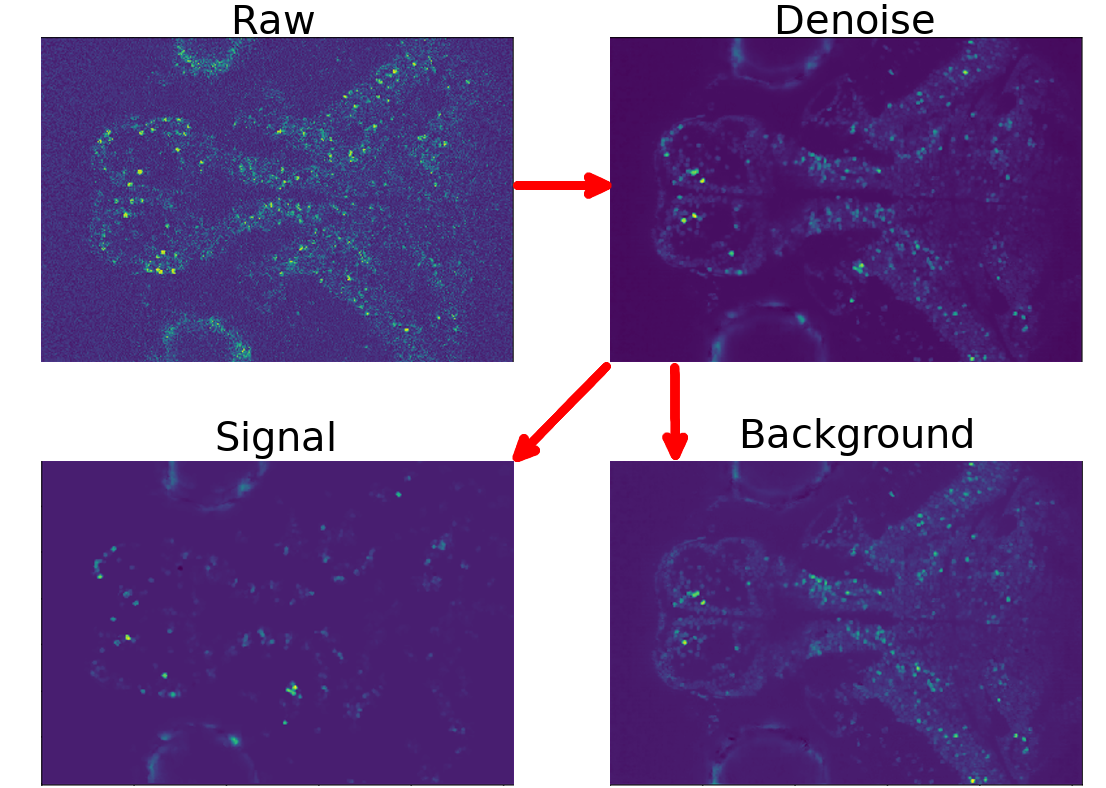
\includegraphics[width=\textwidth]{media/cnmf_arrow.png}
\end{frame}{}

\begin{frame}{Train data: LS and VP perform equally well}{$<5\%$ difference in MSE}
	\centering
	\begin{figure}
		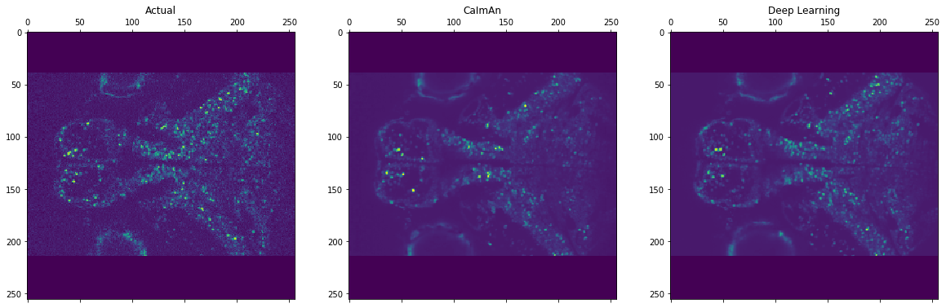
\includegraphics[width=\textwidth]{media/train_mse}
		\caption{Actual (left), least squares prediction (middle), volume prediction (right)}
	\end{figure}
\end{frame}

\begin{frame}{Test data: VP performs better}{LS has 150\% greater MSE than VP}
	\centering
	\begin{figure}
		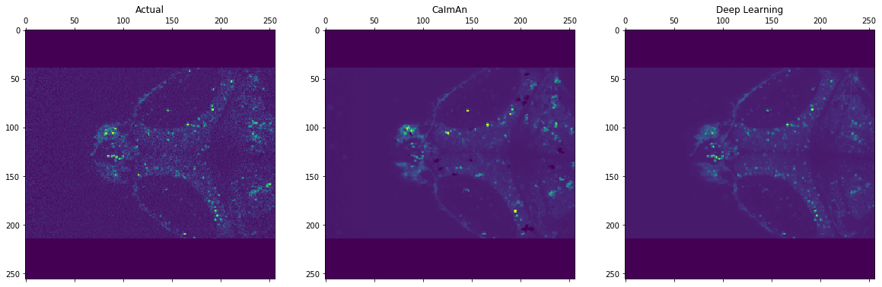
\includegraphics[width=\textwidth]{media/test_mse}
		\caption{Actual (left), least squares prediction (middle), volume prediction (right)}
	\end{figure}

\end{frame}

\begin{frame}{Masked test data: VP performs better}{LS has 40\% greater MSE than VP}
	\centering
	\begin{figure}
		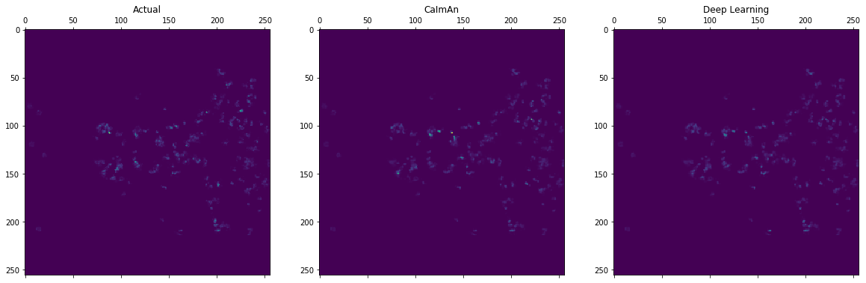
\includegraphics[width=\textwidth]{media/mask_mse}
		\caption{Actual (left), least squares prediction (middle), volume prediction (right)}
	\end{figure}
\end{frame}

\begin{frame}{ CNMF preprocessing reduces VP performance }{Evaluated loss on neuron mask}
	\begin{center}
		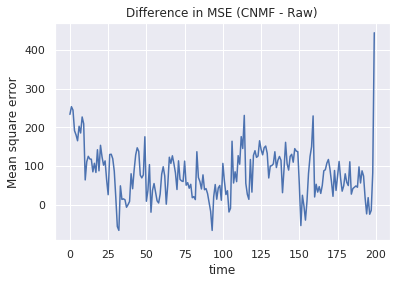
\includegraphics[height=0.7\textheight]{media/cnmf_pairwise.png}
	\end{center}
\end{frame}{}

\begin{frame}{ Extracting causal hypotheses }{Voxels used for predicted locus coeruleus activation}
% TODO
    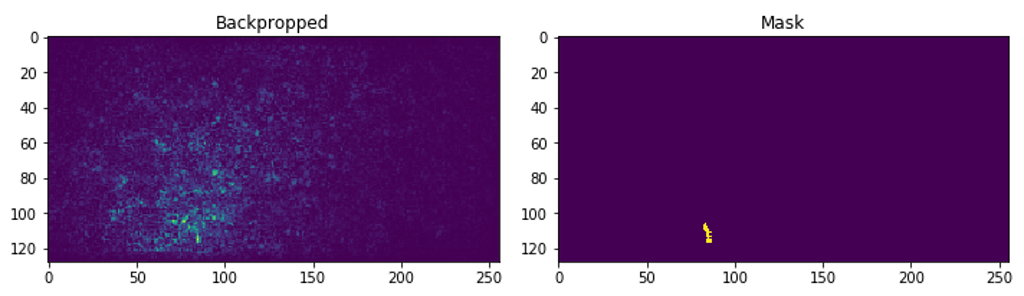
\includegraphics[width=\textwidth]{media/backprop_mask.png}
		\note{Ask model what is important; here we use backprop}
		% \note[item]{ideally show (1) variance heatmap (2) backprop very active neuron (3) backprop very quiet neuron (4) forward autodiff of a neuron (influence mapping)}
\end{frame}{}

\section{\aimTwo}

\note{Active learning, also known as optimal experiment design, is a field that concerns itself with estimating statistical models with as few experiments as possible. Existing literature deals mostly with cases where we can choose exactly what to sample; for example, OED has been deployed in the design of guide RNAs for CRISPR gene editing. In our case, we can only choose the stimuli not the entire brain state. Thus, a causal model will be essential for the penultimate application: brain state replay. }

\begin{frame}{\qTwo}
    \textbf{Hypothesis:} Model-based optimal experiment design will reduce underdetermination
    \begin{itemize}
        \item We can choose optimal optogenetic stimuli to maximally reduce model parameter uncertainty
        \item This can be potentially be done online
        \item We can evaluate how well we have done by attempting to track a brain trajectory
    \end{itemize}
\end{frame}

\begin{frame}{Active learning}{Best to ask for category of which image? }
    \vspace*{\fill}
    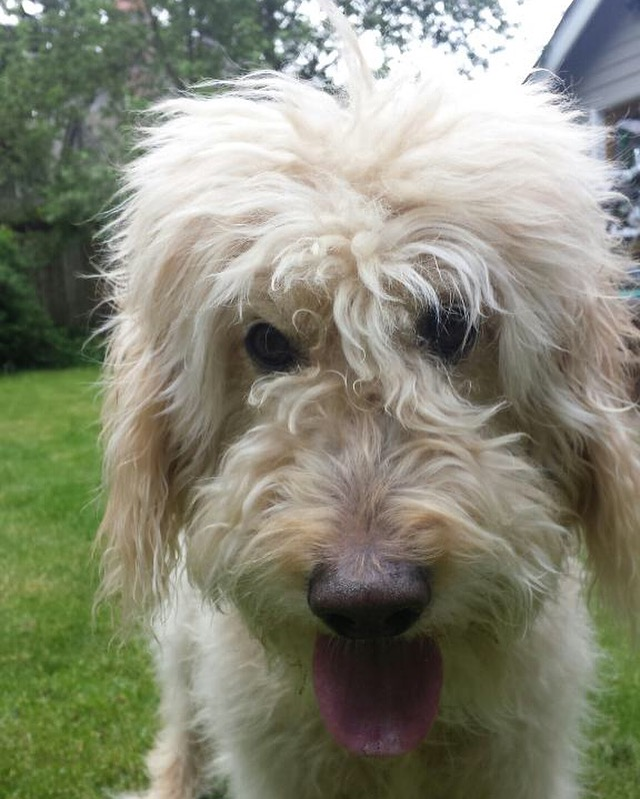
\includegraphics[width=0.31\textwidth]{media/benji.jpg}\nakedfootnote<2>{Mom \& Dad. \emph{personal correspondence}. 2016.}
    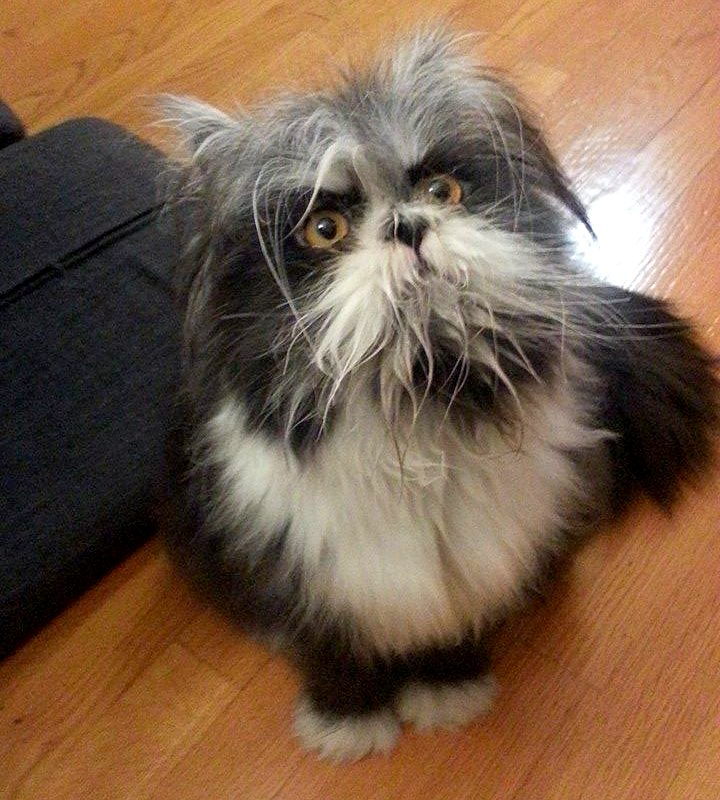
\includegraphics[width=0.31\textwidth]{media/dog-cat}\nakedfootnote<2>{Instagram:atchoumthecat}
    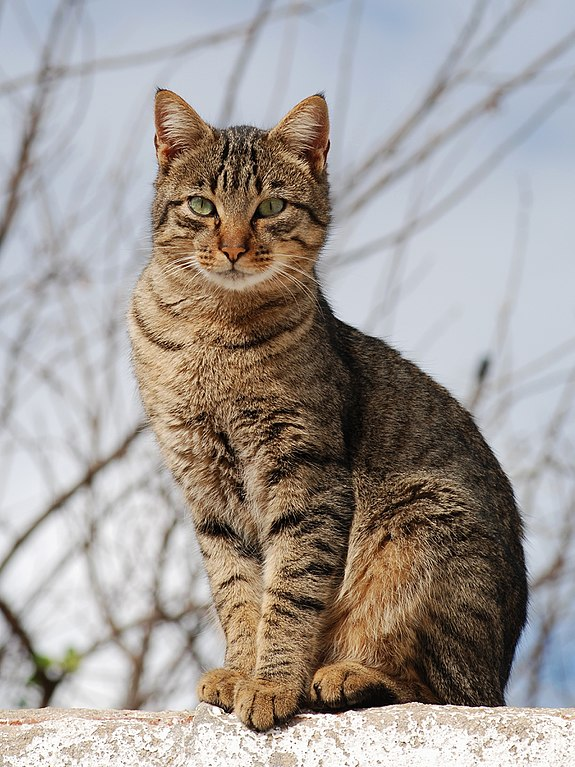
\includegraphics[width=0.31\textwidth]{media/cat}\nakedfootnote<2>{Wikipedia CC BY-SA 3.0}
    \centering
    \uncover<2>{
        \textbf{Cat}
    }
    \note[item]{For which photo would you ask the oracle for a label?}
    \note<2>[item]{Might learn to better use the eyes as a feature}
    \vspace*{\fill}
\end{frame}

\begin{frame}{Interventions resolve model underdetermination}
    \adjincludegraphics[width=\textwidth,trim={{.005\width} 0 0 0},clip]{media/opto-AL.jpg}
    \note{We discuss single neuron stim for intuition. For multi-neuron stim, easier to think in terms of latent space.}
\end{frame}{}

\begin{frame}{Bayesian Active Learning by Disagreement}
    We want to maximize the decrease in expected posterior entropy of model parameters:
    \begin{align}
        \argmax_{s_t} H[\theta|x_{1:t}] - \mathbf{E}_{x_{t+1}}[H[\theta|s_t,x_{t+1},x_{1:t}]]
    \end{align}
    Entropy of model parameters $\theta$ is intractable. So we rearrange to:
    \begin{align}
        \argmax_{s_t} H[x_{t+1}|s_t,x_{1:t}] - \mathbf{E}_{\theta}[H[x_{t+1}|s_t,x_{1:t},\theta]]
    \end{align}
    \nakedfootnote{Houlsby, Huszár, et al. 2011}
\end{frame}

\begin{frame}{Bayesian deep learning via dropout}
    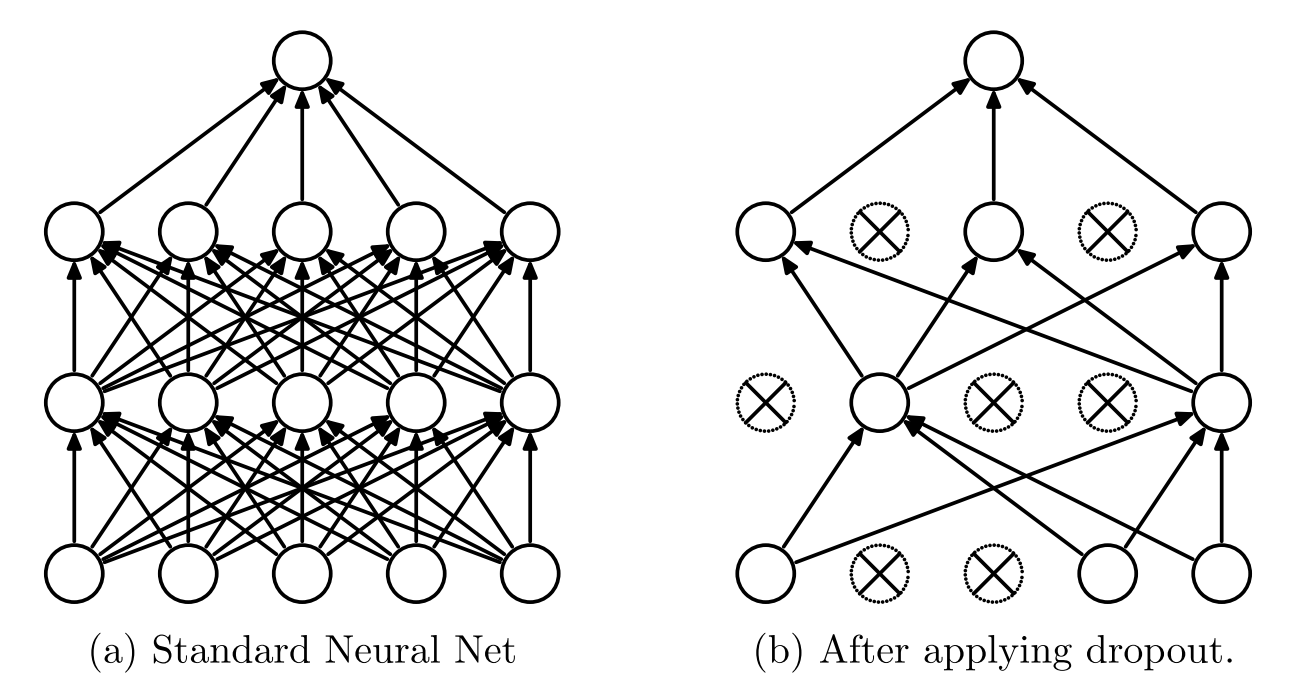
\includegraphics[width=\textwidth]{media/dropout}
    \nakedfootnote{Srivastava, Hinton, et al. 2014}
    \nakedfootnote{Gal 2016}
\end{frame}{}

\begin{frame}{ Collect data then iterate the approach offline }
    Data collection:
    \begin{itemize}
        \item [1] 180 trials of looming stimuli (1 hour)
        \item [2] 360 trials of random single-cell perturbation ( 1 hour)
        \item [3] 180 trials of looming stimuli (1 hour)
    \end{itemize}{}
    Data analysis:
    \begin{itemize}
        \item train on 80\% of trials from [1 \& 3]
        \item choose 60 trials from [2]
        \item Test on witheld trials from [1 \& 3]
    \end{itemize}{}
    How much better can we do by choosing trials vs random trials in terms of test performance?
    \note{This design is mainly to validate our choice of acquisition function (how we choose stimuli) as we can collect all data first then iterate on computational side}
\end{frame}{}

\begin{frame}{ Online optimal experiment design }
    Data collection:
    \begin{itemize}
        \item [1] 225 trials of looming stimuli (1 hour 15 min)
        \item [2] 360 trials, model chooses each single-cell perturbation ( 1 hour)
        \item [3] 225 trials of looming stimuli (1 hour 15 min)
    \end{itemize}{}

    How well can we predict test data by training on 2 hours of looming stimuli vs 1 hour looming \& 1 hour optogenetics?
    \note[item]{Once we've validated offline, can try online. How much can we condense model learning / improve performance?}
    \note[item]{Additional advantage of spatial model is no need for motion correction as convolution is translation invariant. Potential advantage over onACID (online CNMF).}
\end{frame}{}


\begin{frame}{ Brain state replay }
    Data collection:
    \begin{itemize}
        \item [1] Acquire brain trajectory of interest
        \item [2] choose each stimulation pattern sequentially during resting state / experiment of interest
        \item [3] Stim brain to keep observations in line with [1]
    \end{itemize}{}

    How well can we track a previously observed trajectory?

\end{frame}{}

\section{\aimThree}

\note[enumerate]{
    \item Aim 1\&2 are about what we can do with best-in-class models; aim 3 is about simplifying the model / making more biologically compatible. Less complexity but simpler. How close in performance can we get to ``gold standard" model from Aim 1 \& 2?
    \item First, we introduce prior work on functional motif discovery via optogenetics.
    \item Next, I will discuss possible biological priors and constraints
}

\begin{frame}{\qThree}
    \textbf{Hypothesis:} Enforcing causal biological constraints will improve model performance while aiding interpretatation
    \begin{enumerate}
        \item Requiring model to predict \emph{in situ} hybridization allows for interpretation of cell-type contribution to dynamics
        \item Template-based representations allow for unsupervised learning of purported circuit motifs
    \end{enumerate}
\end{frame}

\begin{frame}{ \emph{in situ} cell type identification }
    \begin{center}
        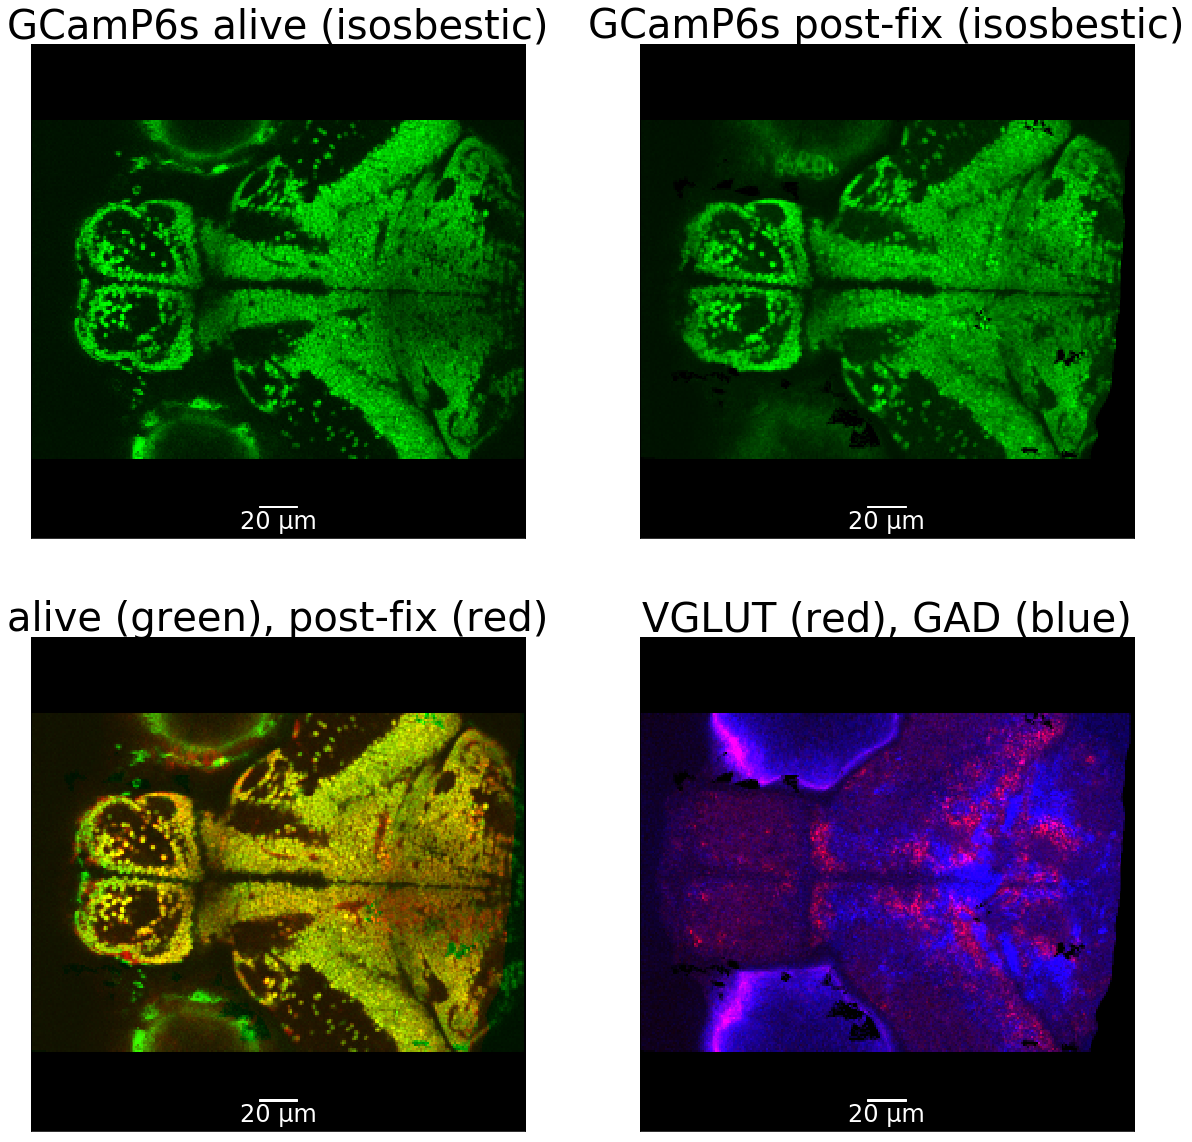
\includegraphics[height=\textheight]{media/ish_stain.png}
    \end{center}
    \note{Talk about colored graphs, predicting cell type,}
\end{frame}{}

\begin{frame}{ Network motifs }
    \begin{multicols}{2}
        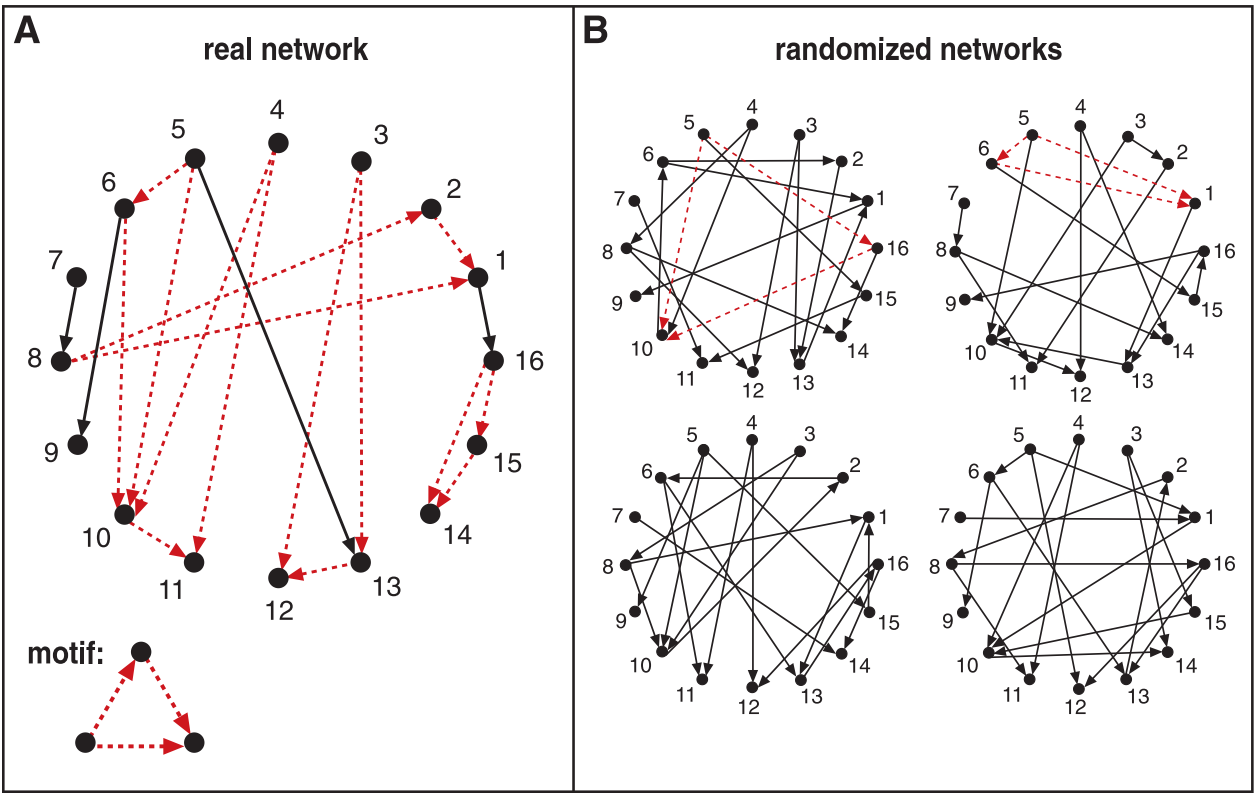
\includegraphics[width=0.5\textwidth]{media/motif_schematic.png}
        Schematic illustrating an over-represented motif\nakedfootnote{Milo et al 2002}
        \note{For a stringent comparison, we used random- ized networks that have the same single-node characteristics as does the real network: Each node in the randomized networks has the same number of incoming and outgoing edges as the corresponding node has in the real network.

        }

        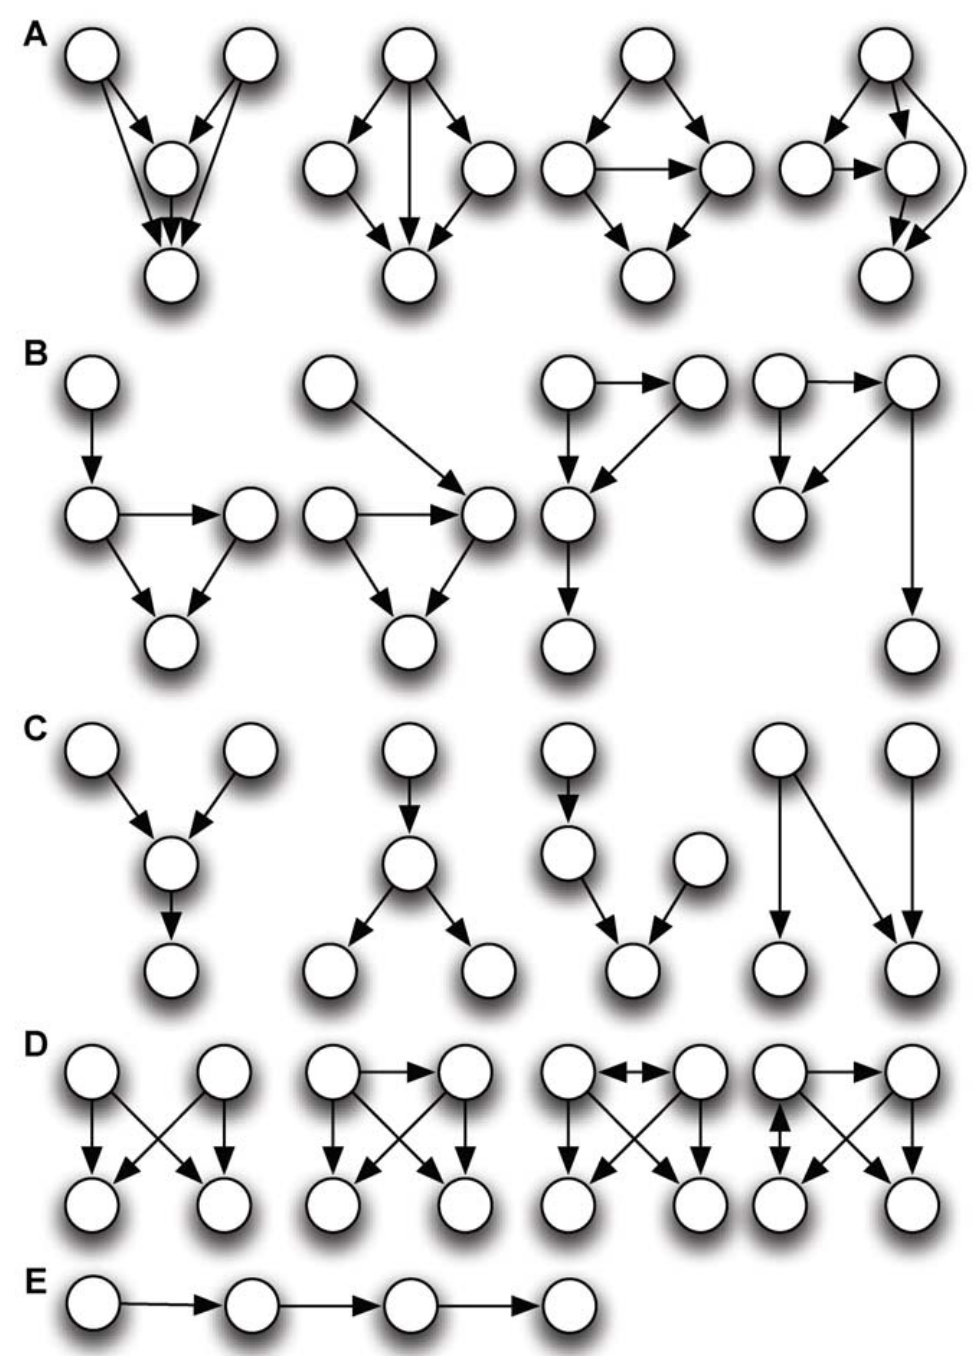
\includegraphics[height=0.7\textheight]{media/celegans_motifs.png}
        Over-represented motifs from \emph{C. elegans} connectome\nakedfootnote{Qian et al 2011}

        \note{A: nested feed-forward motifs, B: feed-forward motifs with entry and exit, C: integrations and bifurcations, D: bi-fan motif with or without coupling of the inputs, and E: linear chains.}
    \end{multicols}
\end{frame}{}

% \subsection{Cell type}
% \subsection{Circuit motifs}


\begin{frame}[t]{Conclusion}
	\begin{itemize}
		\item \aimOne \begin{itemize}
				\item Spatial modeling outperforms point process modeling in prediction accuracy
				\item Next: repeat experiments and analyze tail movement prediction
			\end{itemize}
		\item \aimTwo \begin{itemize}
			\item Established theoretical foundation for selecting optimal optogenetic stimuli to reduce model uncertainty
			\item Next: create transgenic and validate single cell activation
		\end{itemize}
		\item \aimThree \begin{itemize}
			\item Acquired preliminary dataset with co-registered functional imaging and excititory \& inhibitory staining
			\item Next: use model to predict cell type and evaluate influence of cell type on dynamics
		\end{itemize}
	\end{itemize}
\end{frame}

\section{Experiment planning}

\begin{frame}{fishVR V2 Concept}{}
	\centering
	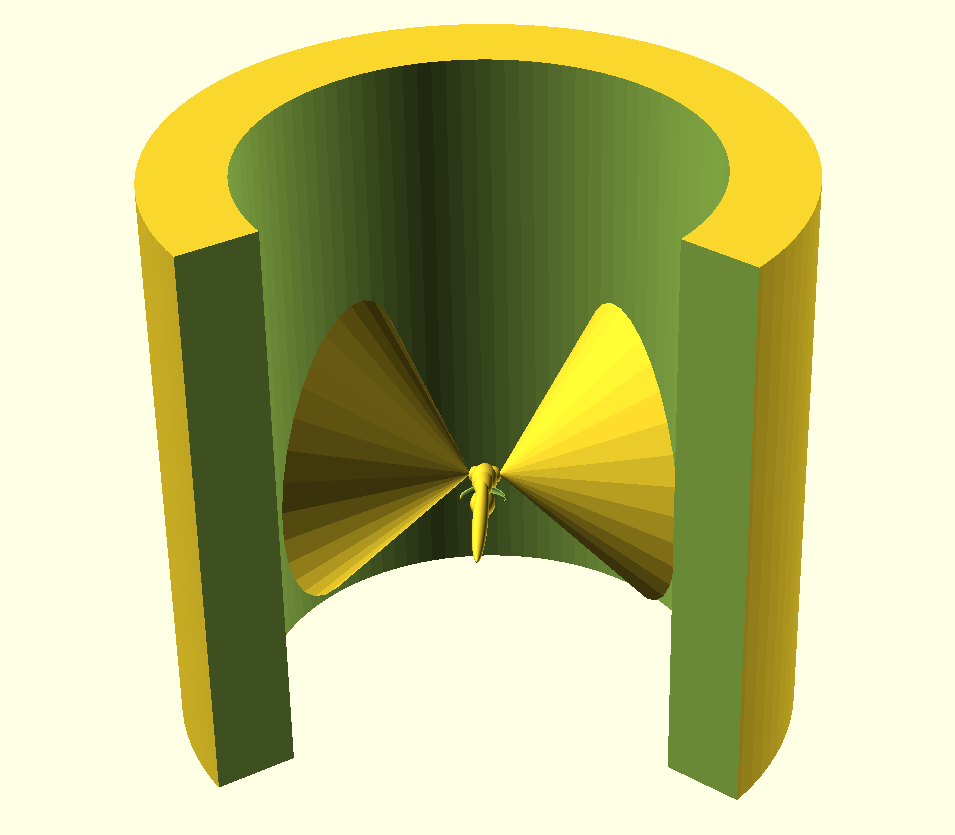
\includegraphics[height=0.9\textheight]{media/zfish_render}\nakedfootnote{https://github.com/BadenLab/Zebrafish-visual-space-model}
\end{frame}{}

\begin{frame}{fishVR V2 Reality}{flexible OLED display}
	\centering
	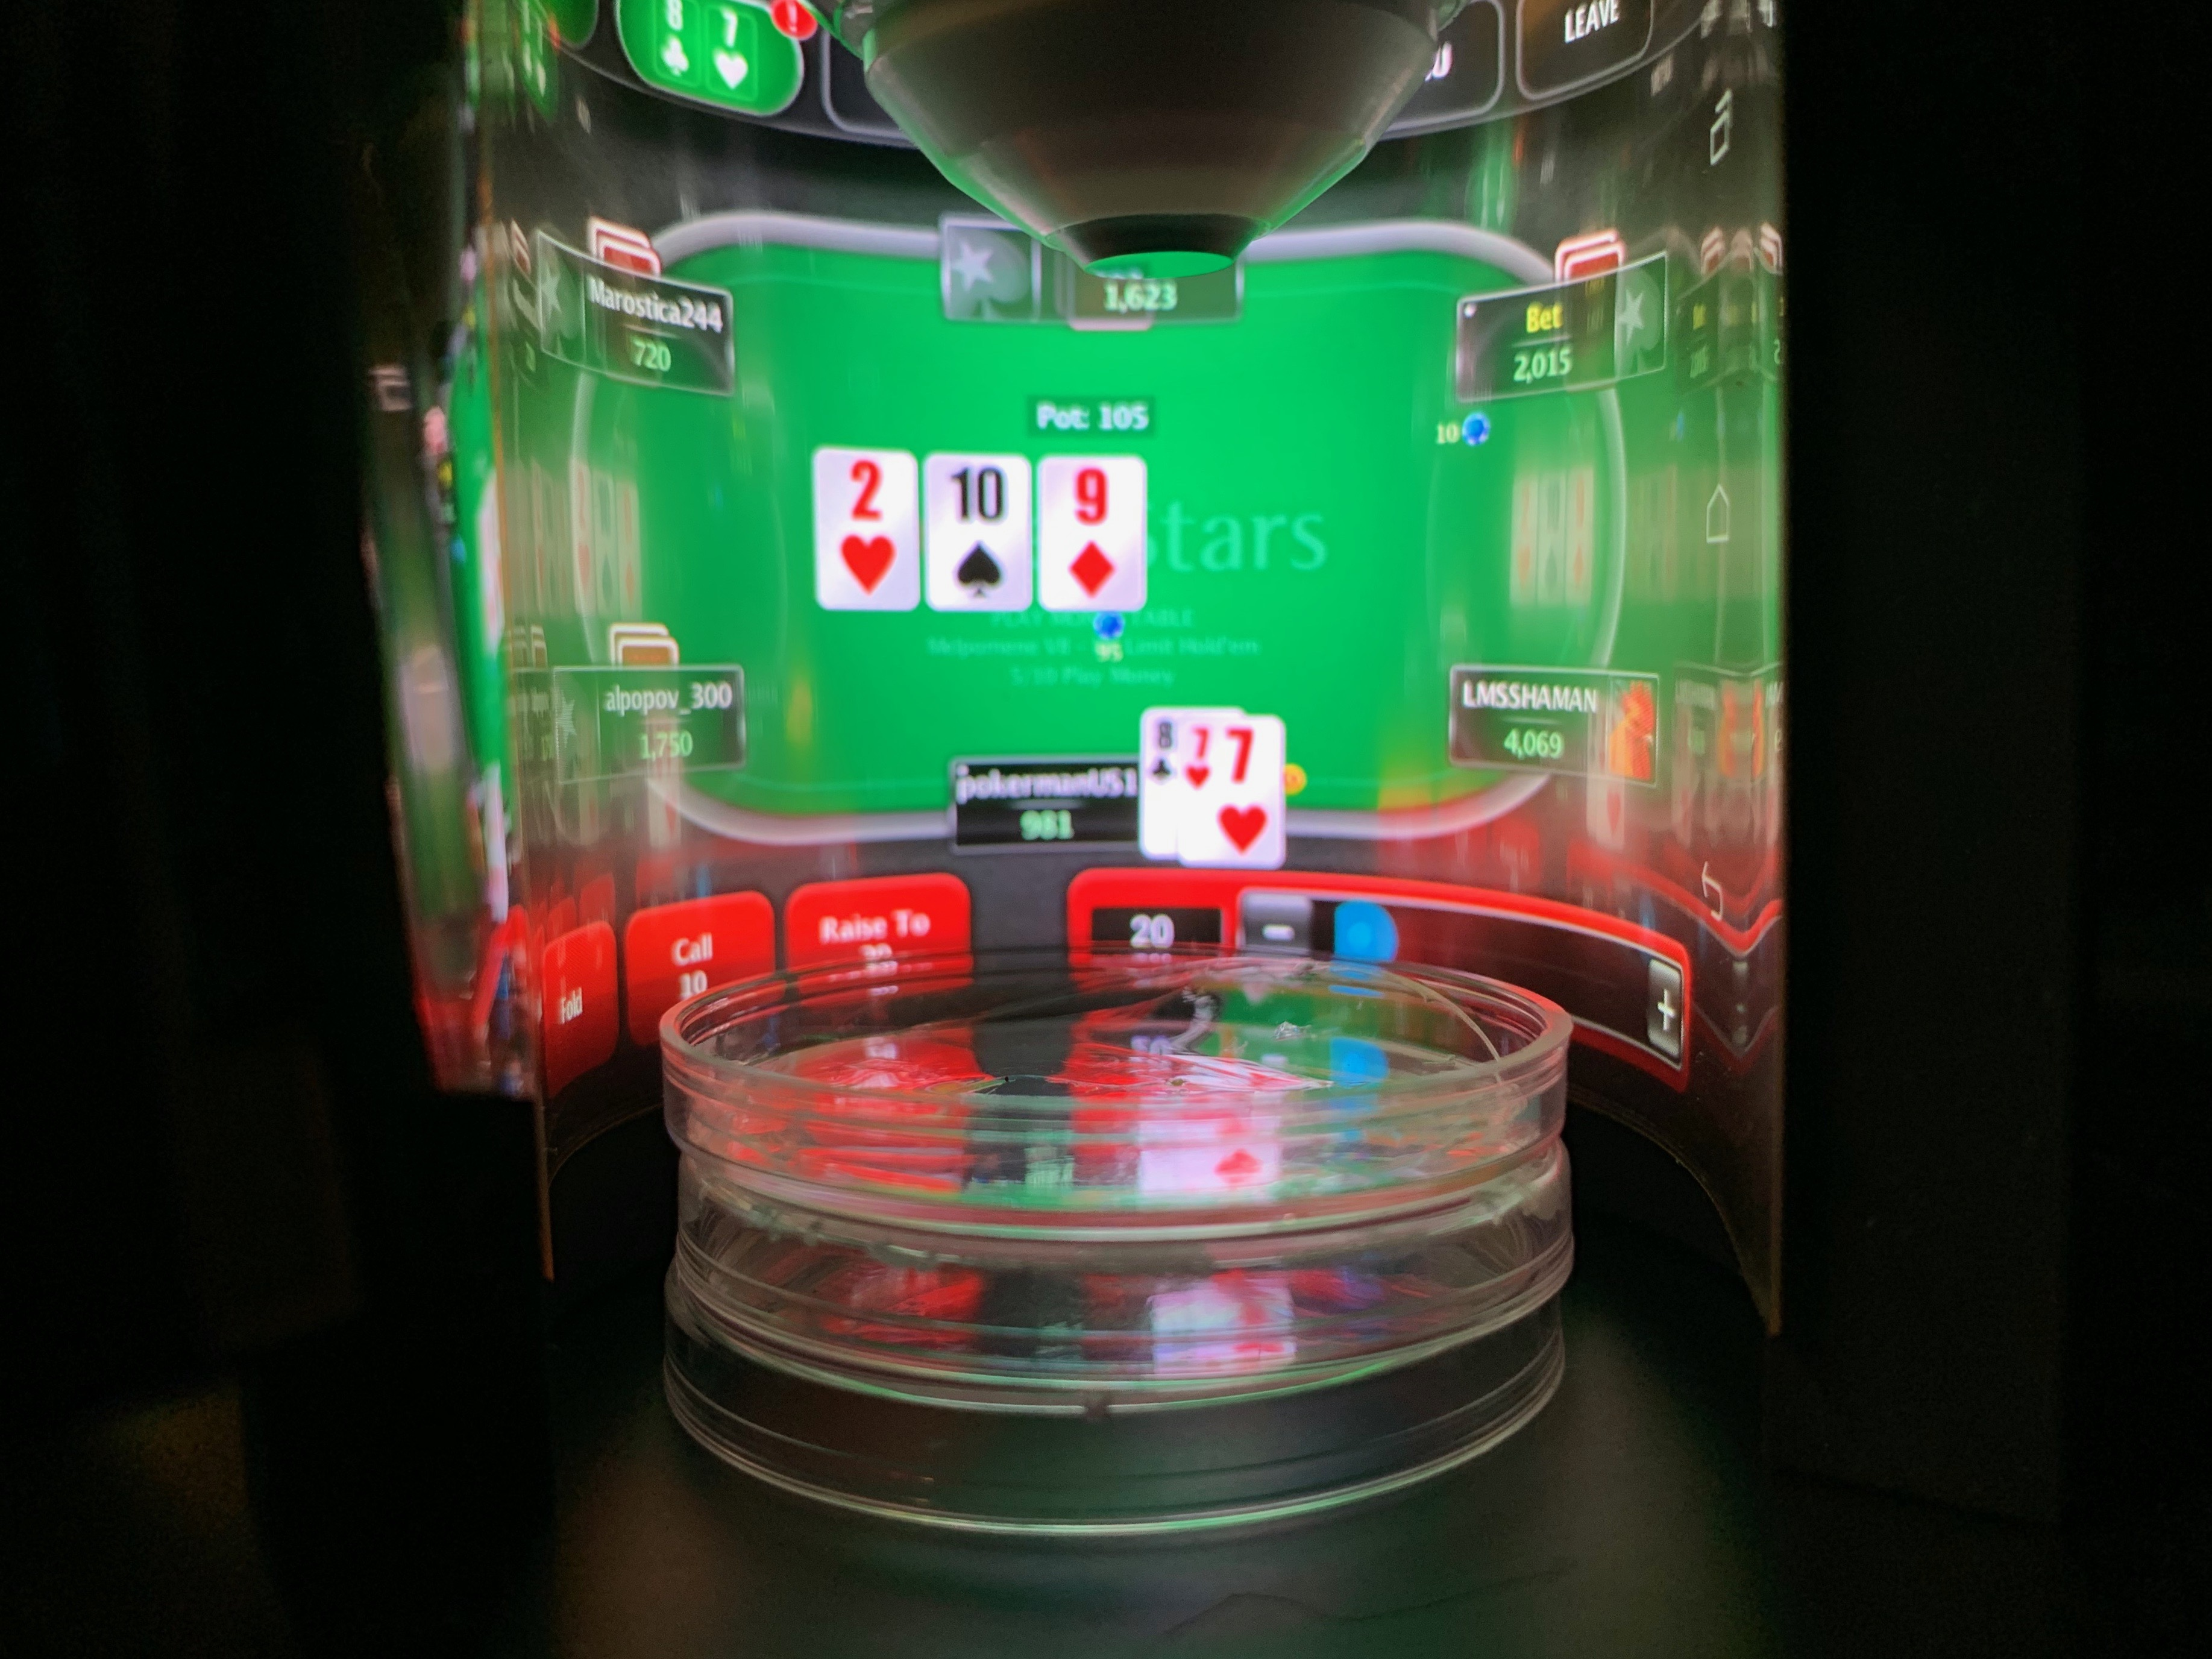
\includegraphics[height=0.9\textheight]{media/poker-fish}
	\note{Unlike LCD and projector, can completely turn off green light}
\end{frame}{}

\begin{frame}{Next steps (feedback welcome!)}{}
	\centering
	\begin{itemize}
		\item Focus on calcium imaging for immediate future \& analyze behavior from optomotor response data
		\item Contextualized passive coping: Aaron's regime with colored queue to indicate if shock is escapable
		\item Pursue initial optogenetic experiments with predicting dynamics recovery after region-wide NpHR inhibition
		\item Outcross F0s in ~1-2 weeks to see if stable F1 emerges
	\end{itemize}
\end{frame}{}

\begin{frame}{Acknowledgements}{}
	\centering
	\begin{columns}[t]
    \column{0.5\textwidth}
			\begin{itemize}
				\item Aaron
				\item Matt LB
				\item Noah
				\item Susanna
				\item Ritchie
				\item YoungJu
				\item Toni
				\item John
				\item Ailey
				\item Sean
				\item Misha, Brian, Ted
			\end{itemize}
    \column{0.5\textwidth}
			\begin{itemize}
				\item Karl
				\item Shaul
				\item Charu
				\item Sally
				\item Cynthia
			\end{itemize}
  \end{columns}
\end{frame}{}


\end{document}
